\htwo{Service Worker}
\sectionauthor{Johannes Polzer}

\hthree{Allgemeines}

Web-Worker sind Javascript-Skripte, die im Hintergrund ausgeführt werden. 
Sie können zum Beispiel dazu verwendet werden, um eine Webseite offline-fähig zu machen oder Push-Notifications zu implementieren.
Da ältere Browser Web-Worker nicht unterstützen (siehe Abbildung \ref{fig:CanIUseServiceWorker}), muss die Kompatibilität vor dem Starten geprüft werden. 
Dazu muss abgefragt werden, ob das "serviceWorker" Objekt in dem "navigator" Objekt existiert. 

\begin{figure}[H]
    \centering
    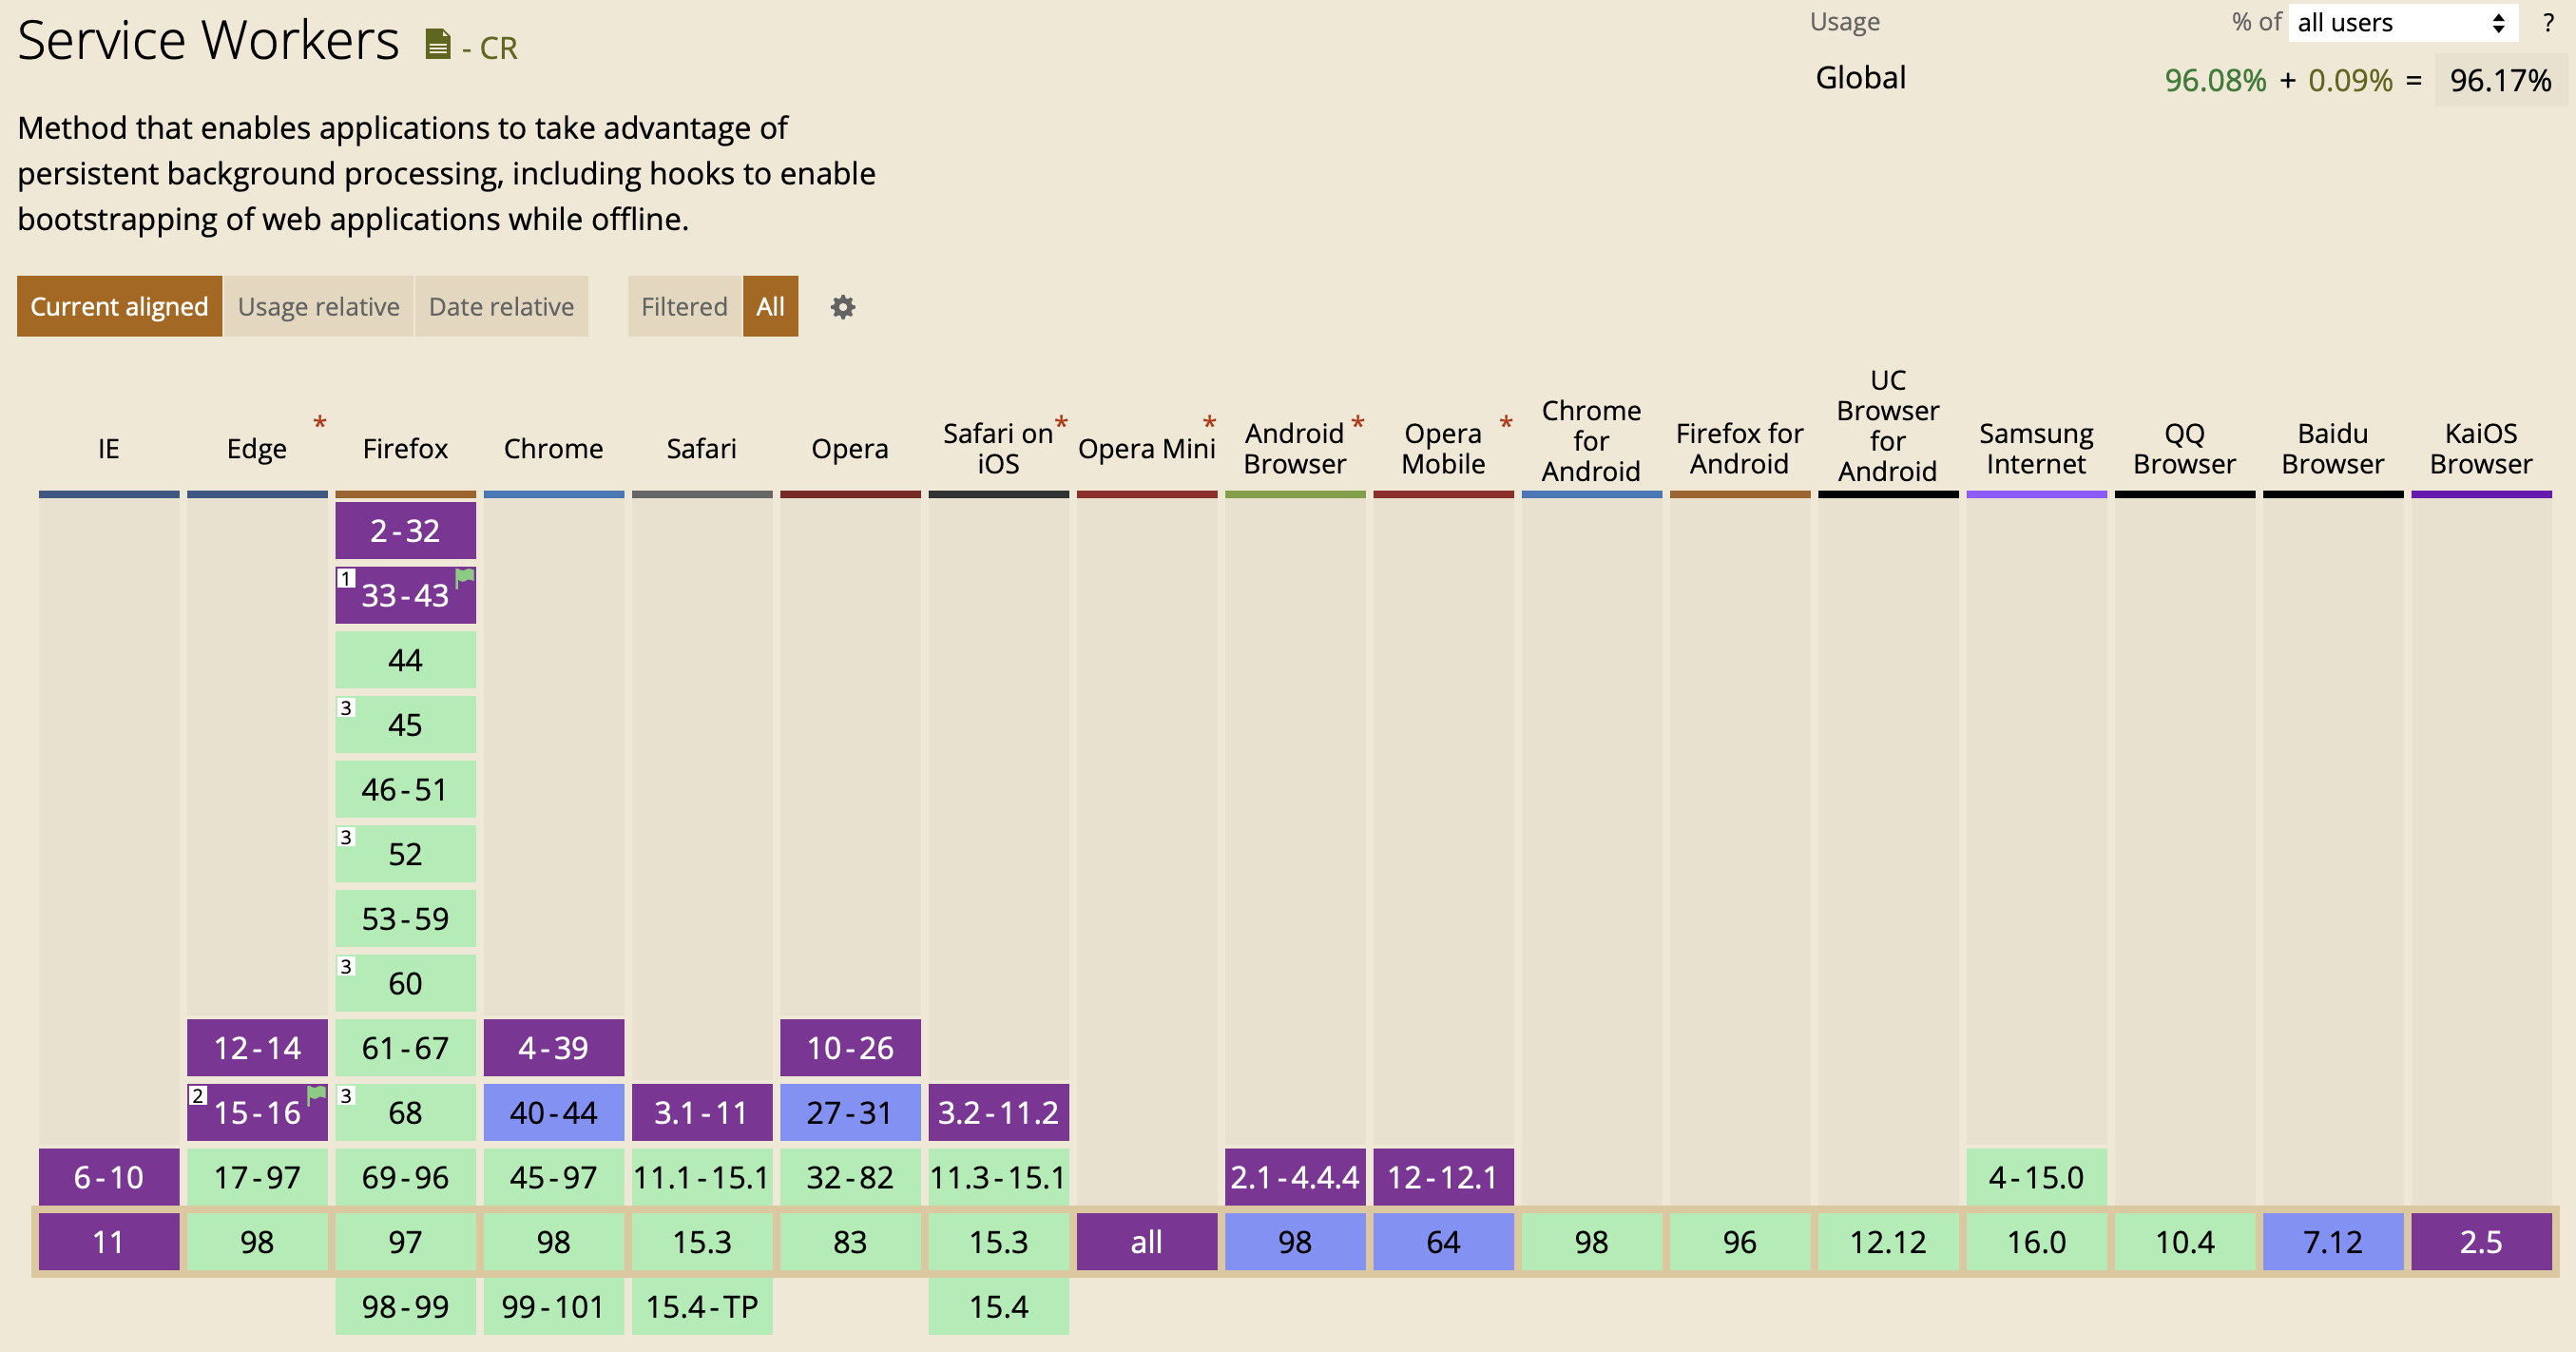
\includegraphics[width=\textwidth]{media/ServiceWorker/CanIUseServiceWorker.png}
    \caption{Eintrag der Unterstützung von Service-Worker in caniuse.com}
    \cite{ciuServiceWorker}
    \label{fig:CanIUseServiceWorker}
\end{figure}

\clearpage

\hfour{Life Cycle Events} 

Ein Service Worker hat verschiedene Events \cite{MDNCacheAPI}: 

\hfive{"Install"-Event}

Das "install"-Event wird ausgelöst, nachdem der Service Worker registriert wurde. Dort werden normalerweise die Abhängigkeiten installiert, \zb\ das Füllen des statischen Cache.
    
\hfive{"Activated"-Event}

Bei der Erstinstallation wird das "activated"-Event unmittelbar nach der Installation ausgelöst.
Wenn ein neuer Service Worker für dieselbe Seite zur Verfügung steht, wird dieser nur installiert.
Die Aktivierung erfolgt jedoch erst in der nächsten Sitzung.
Das "activated"-Event wird in der Regel dazu verwendet, alte Ressourcen aufzuräumen. 
Beispielsweise werden die Caches des vorherigen Service Workers geleert.

\hfive{"Fetch"-Event}

Das "fetch"-Event wird jedes Mal aufgerufen, wenn eine Ressource des Servers angefordert wird. Es fängt diese Anfrage ab, um zum Beispiel mit den Daten aus dem Cache zu antworten.

\hfive{"Push"-Event}

% tofix: Dieser Satz ist komisch
Das "push"-Event wird ausgelöst, wenn der Server ein "push"-Event sendet, welches der Client abonniert hat.

% TODO: gehört da ein kleines h?
\begin{figure}[H]
    \centering
    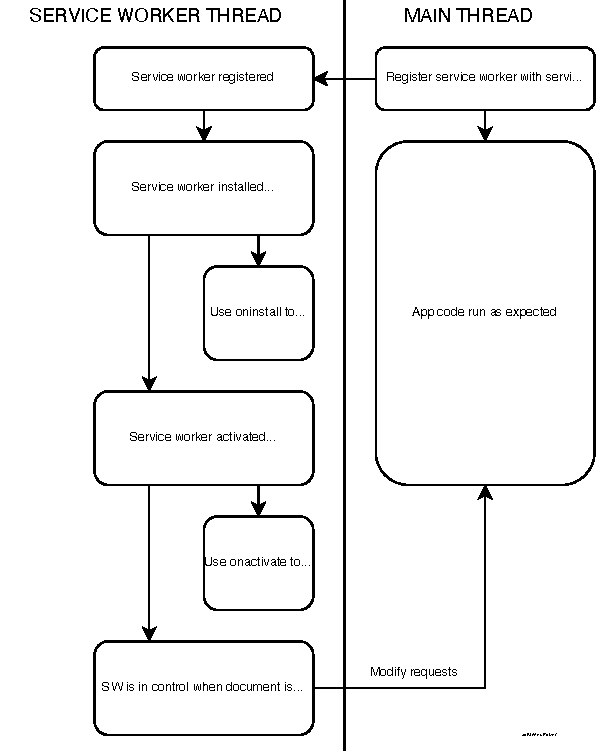
\includegraphics{media/ServiceWorker/lifecycle.svg.pdf}
    \caption{Service Worker Lifecycle}
\end{figure}

\hfour{Registrierung eines Service Workers}

Ein Service Worker kann über das "{\ttfamily serviceWorker}"-Objekt des "{\ttfamily navigator}"-Objekts registriert werden. 
Da Service Worker nicht von allen Browsern unterstützt werden, muss die Kompatibilität vor der Nutzung überprüft werden (um Fehler zu vermeiden).

\typescript{code/ServiceWorker/register.ts}{Registrieren eines Service Workers}

\hthree{Implementierung eines Cache}\label{sec:cacheImpl}

Der folgende Code zeigt, wie ein Service Worker mit der Cache-API zur Verwendung eines statischen und dynamischen Cache-Speichers programmiert wird:

\typescript[code:cache]{code/ServiceWorker/cache.ts}{Verwendung der Cache-API in einem Service Worker}
